\section{Проектирование key-value хранилища}

В данном разделе будет рассмотрен процесс проектирования распределенного key-value
хранилища. Основная цель системы — обеспечить отказоустойчивость и согласованность
данных при репликации за счет алгоритма Raft.

\subsection{Архитектура}

Разрабатываемая система представляет собой распределённое key-value хранилище,
работающее на основе алгоритма консенсуса Raft. Архитектура построена по модели
"лидер-последователь" (master-slave), как показано на рисунке~\ref{fig:fig1} где
один из узлов выполняет роль лидера, а остальные реплицируют его состояние.

\begin{figure}
  \centering
  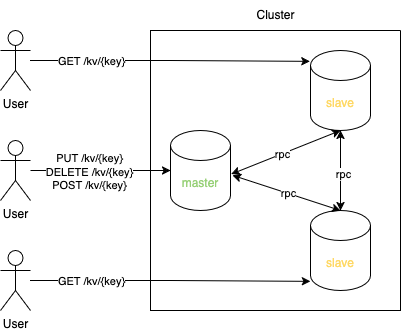
\includegraphics[scale=0.6]{assets/kv_cluster.png}
  \caption{Архитектура key-value хранилища}
  \label{fig:fig1}
\end{figure}

Клиенты взаимодействуют с системой через HTTP API. Операции записи (PUT, DELETE, POST)
отправляются только лидеру, который фиксирует изменения в журнале и распространяет их
на последовательные узлы. Чтение (GET) может выполняться как на лидере, так и на
последовательных узлах, что позволяет балансировать нагрузку.

Обмен данными между узлами осуществляется через бинарный rpc протокол, что обеспечивает
эффективную передачу сообщений и низкие задержки. Последовательные узлы не могут
принимать изменения напрямую, но участвуют в голосовании при выборе нового лидера в
случае сбоя. Лидер принимает запросы на изменение данных и фиксирует их в своём логе.
После этого он рассылает команду обновления состояния всем последователям с
использованием rpc. Узлы подтверждают получение новой записи и добавляют её в свой лог.
Когда большинство узлов кластера подтверждает запись, она считается зафиксированной, и
мастер применяет изменения к своему состоянию, после чего сообщает клиенту об успешном
завершении операции.  

Используемый подход гарантирует согласованность данных и отказоустойчивость, а также
позволяет горизонтально масштабировать систему за счёт добавления новых узлов.

\subsection{Пользовательский API}

Взаимодействие с системой осуществляется через HTTP API, которое предоставляет операции
для управления ключами и значениями. Запросы на изменение данных (`PUT`, `DELETE`)
должны направляться лидеру кластера, в то время как чтение (`GET`) возможно с любого
узла.

\begin{table}[h]
    \centering
    \caption{API кластера KV-хранилища}
    \label{tab:tab1}
    \begin{tabular}{|l|l|l|m{10cm}|}\hline
    \textbf{Метод} & \textbf{URL}       & \textbf{Узел} & \textbf{Описание} \\ \hline
    PUT            & /kv/\{key\}       & Master         & Обновление значения, если он есть и
                                                          создание его в случае отсутствия \\ \hhline{~---}
    DELETE         & /kv/\{key\}       & Master         & Удаление ключа   \\ \hhline{----}
    GET           & /kv/\{key\}       & Slave        & получение значения по ключу     \\ \hline
    \end{tabular}
\end{table}

\subsection{Проектирование конфига}

Конфигурация кластера разработана для обеспечения согласованной работы распределённой
системы на основе алгоритма Raft. Она структурирована в формате YAML, как показано в
листинге~\ref{config}, что обеспечивает человекочитаемость и простоту интеграции с
инструментами автоматизации. Основные разделы и поля конфигурации обоснованы следующими
требованиями:

\listing[
    caption={Пример конфигурационного файла для распределенного кластера},
    label=config
]{assets/config.yml}
